% !TeX spellcheck = de_DE

\documentclass[12pt,a4paper,parskip=half]{scrreprt}

\usepackage[english]{babel}
\usepackage[utf8]{inputenc}
\usepackage{acronym}
\usepackage{graphicx}
\usepackage[below]{placeins}
\usepackage{url}
\usepackage{hyperref}
\usepackage{tabularx}
\usepackage{booktabs}
\usepackage{textcomp}
\usepackage{caption}

% font coloring
\usepackage{xcolor}
% for tables
\usepackage{multirow}

\newcommand*{\captionsource}[2]{%
	\caption[{#1}]{%
		#1%
		\\\hspace{\linewidth}%
		\textbf{Quelle:} #2%
	}%
}

\title{Bericht Praxisphase I}
\author{Sebastian Wallat}
\date{\today}

\clubpenalty = 10000 % schliesst Schusterjungen aus
\widowpenalty = 10000 % schliesst Hurenkinder aus

\graphicspath{{./images/}}

\begin{document}

\begin{titlepage}
	
	\centering
	
%%	\ifcsempty{iodhbwm@institute@logo}{%
		
%%		
\includegraphics[height=1.5cm]{dhbw-logo}
		
	{%
		
		\begin{minipage}[c]{.25\textwidth}
			
			
\includegraphics[width=\textwidth, height = 2cm]{dhbw-logo}
			
		\end{minipage}
		\begin{minipage}[c]{0.46\textwidth}
			
			
\includegraphics[width=\textwidth]{empty}
			
		\end{minipage}
		\begin{minipage}[c]{.25\textwidth}
			
			\raggedleft
			
			
\includegraphics[width=\textwidth, height =2cm, keepaspectratio]{dlr-logo}
			
		\end{minipage}
		
	}
	
	
	
	\bigskip
	
	
	
	\Large\textsc{Große Studienarbeit}
	
	
	
	\normalsize
	
	des Studiengangs Informationstechnik\par
	
	der Dualen Hochschule Baden-Württemberg Mannheim
	
	
	
	\rule{\textwidth}{.5mm}\bigskip
	
	
	
	\textsc{\large Performance Analysis of serverless cloud functions}	
	
	
	\rule{\textwidth}{.5mm}
	
	
	
	\vfill
	
	
	
	\par
	
	{\bfseries\large Sebastian Wallat}\par
	
	\today
	
	
	
	\vfill
	
	
	
	\small{%
		
		\begin{tabularx}{\textwidth}{@{}lX@{}}
			
			\toprule
			
			
			Bearbeitungszeitraum: & 24.10.2020-27.11.2020\\
			
			Matrikelnummer, Kurs: & 1708267, TINF18-IT1\\
			
			Beteuer: & Dr. Frank Schulz \\
			
		\end{tabularx}
		
	}
	
	\cleardoublepage
	
\end{titlepage}


\newpage
\pagenumbering{Roman}

\chapter*{Eidesstattliche Erklärung}
%%\thispagestyle{empty}
\vspace{50pt}
TODO
\\
\\

\vfill
\noindent\rule{5cm}{.4pt}\hfill\rule{5cm}{.4pt}\par
\noindent Datum, Ort \hfill Unterschrift 

\newpage
\thispagestyle{empty}
\chapter*{Zusammenfassung}

 Performance Analysis of serverless cloud functions
\\
\bigskip


\tableofcontents
\addtocontents{toc}{}

\listoffigures
\addcontentsline{toc}{chapter}{Abbildungsverzeichnis} 
%%\thispagestyle{empty}

\newpage
\chapter*{Abkürzungsverzeichnis}
\addcontentsline{toc}{chapter}{Abkürzungsverzeichnis}
%%\thispagestyle{empty}
\begin{acronym}[HTTP]
	\acro{DLR}{\textbf{D}eutsches Zentrum für \textbf{L}uft- und \textbf{R}aumfahrt}
	\acro{SaaS}{\textbf{S}oftware-\textbf{a}s-\textbf{a}-\textbf{S}ervice}
	\acro{CAD}{\textbf{C}omputer-\textbf{A}ided \textbf{D}esign}
	\acro{CSP}{\textbf{C}loud \textbf{S}ervice \textbf{P}rovider}
	\acro{AWS}{\textbf{A}mazon \textbf{W}eb \textbf{S}ervices}
	\acro{SLA}{\textbf{S}ervice \textbf{L}evel \textbf{A}greements}
\end{acronym}

\pagenumbering{arabic}

\chapter{Einführung}
Durch die stetig voranschreitende Digitalisierung von Unternehmen gewinnen im Besonderen Cloud-Basierte Softwarelösungen an Bedeutung. Hierzu zählen unter anderem Software-as-a-Service (SaaS) Angebote wie Office356 von Microsoft (Textverarbeitung) oder Fusion360 von Autodesk (CAD-Programm). Des weiteren sind auch der Großteil (NEEDS PROOF) der heutigen Web-Anwendungen in der Cloud gehostet.  Alle diese Anwendungen haben gemein, dass die wesentliche Datenverarbeitung nicht auf dem Gerät des Nutzers erfolgt, sondern auf den Servern des Cloud Service Provider (CSP). Hierfür bieten die meisten CSP Baukastensysteme an um schnell komplexe Backend-Strukturen innerhalb ihrer Umgebung implementieren zu können. Einige Bespiele hierfür sind Datenbanksysteme, API-Gateways, Serverlose-Funktionen, (Container)-Hosting und weitere.
\\
Das Ziel dieser Arbeit ist es sich mit einem dieser Systeme näher zu beschäftigen, den Serverlosen Cloudfunktionen. Diese bieten die meisten CSP in ihrer Infrastruktur an, z.B AWS-Lambda (Amazon Web Services) und Google Cloud Run.
\\
Cloudfunktionen sind eine kostengünstige Lösung um bestimmte Backend Funktionalitäten zur Verfügung zu stellen. Sie sind zustandslose (stateless) Programmstücke, die über eine definierte Aktion aktiviert werden, z.B einen API Aufruf. Zur Ausführung erstellt der CSP einen neue Instanz der Funktion (falls nicht schon vorhanden) und führt diese aus. Die Besonderheit hierbei ist die zustandslösigkeit, also die Eigenschaft der Funktion keine persistenten Daten zu speichern. Alle für die Ausführung benötigten Daten, müssen vom Aufrufer mitgegeben werden, oder aus einer persistenten Datenquelle (z.b Datenbank) geladen werden. Da die Funktion aus diesem Grund nicht auf einem normalen Webserver läuft, sondern nur führ einen Aufruf existiert, werden sie auch als serverlos bezeichnet.
\\
Der größte Vorteil von Cloudfunktionen gegenüber einem herkömmlichen Webserver, liegt darin, dass nur pro Aufruf kosten einstehen. Da ein normaler Webserver ja durchgängig Ressourcen des CSP belegt, fallen für ihn auch kosten an, wenn er nicht benutzt wird.
\\
Aus diesem Verhalten ergibt sich direkt auch ein wesentlicher Nachteil, der allerdings die meisten Cloud-Services betrifft, dieser liegt in der Varianz der Kosten. Erfreut sich ein Service unerwarteter Beliebtheit, so können unerwartet hohe Kosten durch den vermehrten Aufruf der Funktion entstehen.
\\
Dies wird besonders durch die gute horizontale Skalierbarkeit der Cloudfunktionen verstärkt. Würde ein traditioneller Webserver durch zu viele Anfragen überlastet, kann man von einer Funktion beliebig viele Instanzen erzeugen, welche die Anfragen parallel verarbeiten können.
\\
\\
Im weiteren Verlauf der Arbeit kann aus mehreren Gründen nur auf einen CSP eingegangen werden, hierfür wurde AWS ausgewählt. AWS stellt Cloudfunktionen unter seinem AWS-Lambda Service bereit. Daher sind die folgenden Ausführungen nur in der AWS Umgebung gültig und die präsentierten Resultate gelten nur für AWS-Lambda Funktionen.
\cite{Lambda-overview} 

\chapter{Technischer Hintergrund (AWS Lambda)}
AWS beschreibt Lambda folgendermaßen: "AWS Lambda ist ein serverloser Datenverarbeitungsservice, der Ihren Code beim Eintreten bestimmter Ereignisse ausführt und für Sie automatisch die zugrunde liegenden Datenverarbeitungsressourcen verwaltet" \cite{Lambda-overview}
\\
Dies lässt sich an einem kleinen Beispiel verdeutlichen:
\FloatBarrier
\begin{figure}[h!]
	\centering
	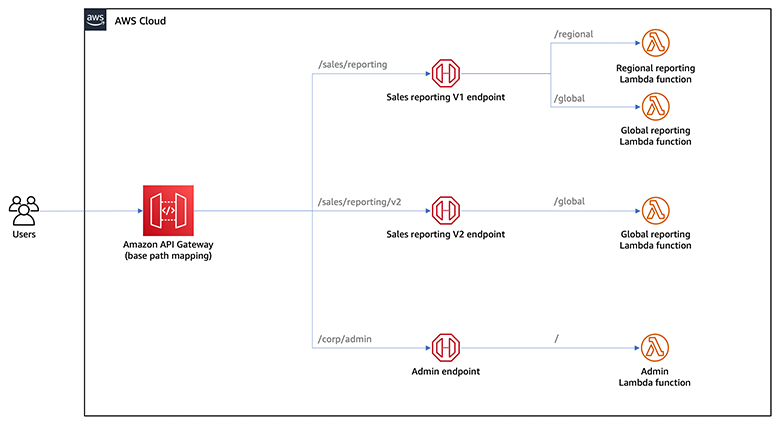
\includegraphics[width=14cm, height=8cm]{LambdaExample}
	\captionsource{Beispiel für den Einsatz von Lambda Funktionen mit einem API-Gateway als Auslöser}
		{https://aws.amazon.com/de/blogs/compute/icymi-serverless-q1-2021/}
	\label{AWS_Example}
\end{figure}

Grafik \ref{AWS_Example} zeigt die Verwendung von Lambda Funktionen in Kombination mit einem AWS API Gateway. Der Gateway besitzt mehrere vordefinierte Endpunkte, die jeweils mit einer Lambda-Funktion verknüpft sind. Schickt ein Nutzer eine HTTP Anfrage mit einem bestimmten Pfad (z.B ''/corp/admin'') an den die URL des API Gateway, so extrahiert dieser den konkreten Pfad der Anfrage und startet die verknüpfte Lambda-Funktion (in diesem Fall die ''Admin'' Funktion).

\chapter{Performance Tests}

Ziel soll es sein AWS Lambda Funktionen auf ihre Performanz zu untersuchen. Als Kriterien hierfür bieten sich Latenz und Verfügbarkeit an.
\\
In den Service Level Agreements (SLA) von AWS Lambda garantiert AWS eine Verfügbarkeit von mindestens 99.95\% pro Monat. Sollte dies nicht erfüllt werden, so bekommt der Kunde eine Gutschrift für zukünftige Lambda Kosten, in Form sogenannter ''Service Credits''. Ab einer Verfügbarkeit von unter 95\% werden die gesamten Kosten als Service Credits gutgeschrieben.
\cite{Lambda-SLA}
\\
Weitere Informationen hierzu findet man in der offiziellen SLA von AWS Lambda (\url{https://aws.amazon.com/de/lambda/sla/})
\\
Da die Angaben der SLA dafür sprechen dass AWS von einer hohen Verfügbarkeit ausgeht und dies bei einem weltweit führenden CSP durchaus erwartet werden kann, soll die Verfügbarkeit nicht Fokus der weiteren Untersuchungen sein.
\\
Da die Lambda SLA keine Angaben zur Latenz machen, soll diese näher untersucht werden. Besonders die Problematik des sogenannten ''Cold start'' (zu deutsch Kaltstart) soll untersucht werden.

\section{Cold start (Kaltstart) von serverlosen Architekturen}
Aufgrund der serverlosen Architektur von AWS Lambda liegt die Vermutung nah, dass er Kaltstart wesentlichen Anteil an der Latenz einer Lambda Funktion haben könnte. Daher soll zuerst geklärt werden worin genau die Kaltstart-Problematik besteht.
\\
Da Lambda keinen permanenten Server Prozess besitzen, existieren zu einer bestimmten Zeit t eine bestimmte Anzahl n von Instanzen der Funktion. Wie groß n zu einem konkreten Zeitpunkt ist, wird von Skalierungsalgorithmen bestimmt und hängt in erster Linie von der Anzahl der Aufrufe in einem bestimmten Zeitfenster $\Delta$t ab. (vgl. Autoscaling von AWS Lambda).
\\
Um Kosten zu sparen wird die Anzahl der Funktions-Instanzen auf null reduziert, falls in einem festgelegten Intervall keine Aufrufe der Funktion stattfinden.
\\
Trifft nun ein neuer Aufruf für die Funktion ein, so muss der CSP zuerst eine neue Instanz erstellen, welche dann die Anfrage bearbeiten kann. Dies wird als Kaltstart bezeichnet (Skalierung von $n=0$ auf $n\geq1$)
\\
Die Gesamtzeit des (oder der) ersten Funktionsaufrufe(s) erhöht sich somit um die Zeit, die zur Instanziierung der Funktion benötigt wird. Je nach verwendeter Programmiersprache kann es passieren dass das Programm deutlich langsamer Ausgeführt wird als nach einiger Laufzeit (z.B JIT Laufzeitoptimierung von Java). In diesem Fall vergrößert sich die Laufzeit nach Kaltstart zusätzlich.

\section{Testaufbau}
Um verschiedene Performance-Aspekte von AWS Lambda Funktionen zu untersuchen wurde folgender Testaufbau verwendet.

\subsection{AWS}

Der Testaufbau besteht aus 4 in AWS implementierten Lambda-Funktionen. Diese sind über einen API Gateway erreichbar.

\FloatBarrier
\begin{figure}[h!]
	\centering
	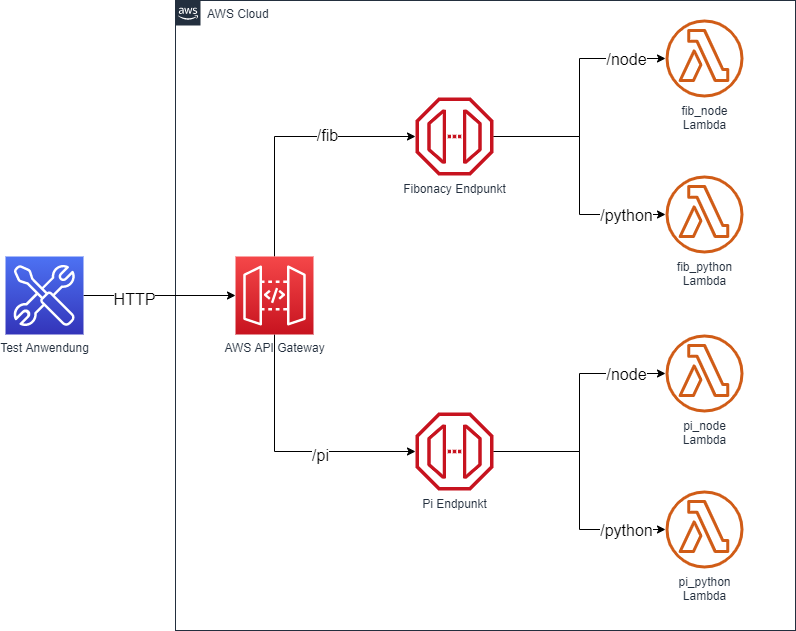
\includegraphics[width=14cm, height=10cm]{LambdaLayout}
	\captionsource{Beispiel für den Einsatz von Lambda Funktionen mit einem API-Gateway als Auslöser}
	{Eigene Darstellung mit DrawIO}
	\label{Lambda_Aufbau}
\end{figure}

Darstellung \ref{Lambda_Aufbau} zeigt eine Überblickskizze über die in der Cloud-Implementierten Funktionalitäten. Insgesamt wurden vier Lambda-Funktionen implementiert, hierbei wurden zwei verschiedene Programmiersprachen und zwei Arten von Workloads berücksichtigt. Als verwendete Sprachen werden Python und Java Script (NodeJS-Framework) verwendet. Bei den implementierten Workloads handelt es sich einmal um die iterative Berechnung von $\pi$ auf eine festgelegte Anzahl stellen, sowie um die rekursive Berechnung einer Zahl der Fibonacci folge. Der Sourcecode kann unter folgendem Link eingesehen werden: \url{https://github.com/SebastianWallat/StudienarbeitAWS}
\\
Des weiteren dokumentiert jede Lambda Funktion ihre Laufzeit und sendet diese, sowie das Ergebnis der Berechnung an den Aufrufer zurück.


\subsection{Test-Anwendung}

Um die zuvor implementierten Lambda-Funktionen zu testen wurde eine einfache NodeJS Anwendung entwickelt. Diese aktiviert die Lambda-Funktionen über ihre korrespondierenden API-Pfade und speichert die Ergebnisse als CSV. Die Sequenz der Aufrufe wird in einer CSV Datei festgelegt und steuert das Timing der Anwendung.

\section{Auswertung}

Zur Auswertung der so generierten CSV Datei wird ein Jupyter-Notebook (Python) verwendet, dieses visualisiert die Latenzzeiten unter Verwendung der üblichen Data-Science Frameworks (unter anderem Pandas, Matplotlib).




\newpage

\nocite{*}
\thispagestyle{headings}

\bibliographystyle{IEEEtr}
\bibliography{bibo} 

\end{document}